% ps3-reinforcement.tex
\documentclass{article} %The basic layout of the output document, sets things like pagesize and defaults
\usepackage{amsmath} %a package for good looking equations and symbols
\usepackage{algorithm2e} %a package for typesetting algorithms
\usepackage{caption} %a package for more complex captions for figures/tables/images
\usepackage{subcaption} %extension of the caption package
\usepackage{url} %embedded, clickable links
\usepackage{fullpage} %including this package changes the default margins to use more of the page
\usepackage{graphicx} %package for inline images
\usepackage[usenames]{xcolor} %for adding color text
\usepackage{enumitem} %for nested numbered lists (like in the questions section)

%note that the title and date are specified /before/ the "\begin{document}" command.
\title{Introduction to Artificial Intelligence\\ %double backslash (ie, "\\") are typically used to force a newline in most environments
Problem Set 3 --- Reinforcement Learning}
\date{} %an empty string "{}" is OK here, but some environments/commands will throw an error.
\author{}

\begin{document}
\maketitle %The "\maketitle command" is what actually formats and inserts this information into the text.

%some latex magic that creates a new command for use in this document. This particular command is handy for annotating
%changes or temporary text.
\newcommand{\bphnote}[1]{\textit{\textcolor{red}{#1}}}


\section*{Instructions} %Sections and subsections create headers and are automatically numbered
In this problem set we're going to run through value iteration and Q-Learning by hand. 

\section*{Questions}
For the next few questions, use the environment described in figure \
\begin{figure}
\begin{center}
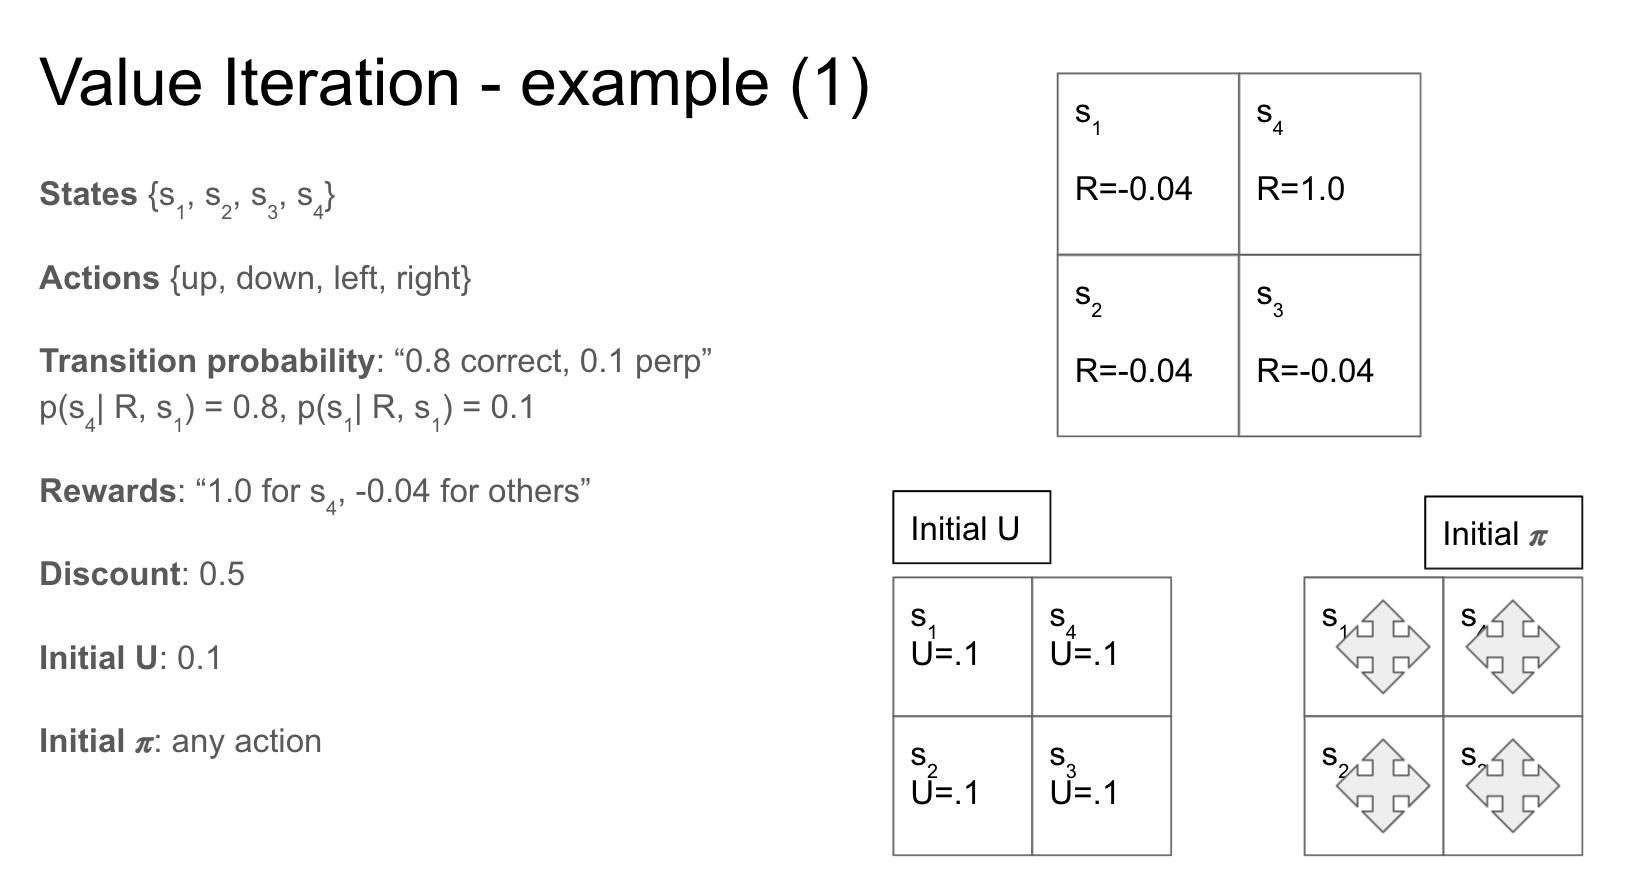
\includegraphics[height=0.3\textheight]{2x2-gridworld}
\caption{A tiny gridworld.}
\label{2x2-gridworld}
\end{center}
\end{figure}

\begin{enumerate}
\item Run Value Iteration \emph{by hand} for 10 iterations on the given environment. Make sure you note down the utility at each iteration separately to keep things organized.
\item Write some code to automate the utility updates for this environment. Make sure your code agrees with the work you did by hand in the previous question.
\item How long does it take for the utility to converge? Pick a threshold for small differences and see how long it takes until none of the utility values for any of the states is changing more than this threshold.
\item Run Q-Learning by hand on the same environment using a learning rate of \(\alpha=0.5\), an initial Q-table of all zeros, and the following experience traces (given as \((s, a, s^\prime, r)\) tuples):
	\begin{enumerate}
		\item \((s_2, Up, s_1, -0.04)\)
		\item \((s_1, Right, s_4, 1.0)\)
		\item \((s_2, Right, s_3, -0.04)\)
		\item \((s_3, Up, s_2, -0.04)\)
		\item \((s_2, Up, s_1, -0.04)\)
		\item \((s_1, Right, s_4, 1.0)\)
	\end{enumerate}
\item Assuming that the world resets after the agent visits state \(s_4\), and the agent starts in state \(s_2\), do these experience traces suggest that this is a greedy agent? Why or why not?
\item If a greedy agent were being used to generate experience traces for Q-Learning in this environment, would we be guaranteed to visit every state (in the limit)? What single aspect of the environment could be changed to flip your answer (yes to no, no to yes)?
\end{enumerate}

\section*{Submission}
Write up your answers to the given questions as a single PDF file, and put any code into a single python file.

\end{document}